\documentclass[12pt,a4paper]{article}
\usepackage{ctex}
\usepackage{amsmath,amscd,amsbsy,amssymb,latexsym,url,bm,amsthm}
\usepackage{epsfig,graphicx,subfigure}
\usepackage{enumitem,balance}
\usepackage{wrapfig}
\usepackage{mathrsfs,euscript}
\usepackage[usenames]{xcolor}
\usepackage{hyperref}
\usepackage[vlined,ruled,linesnumbered]{algorithm2e}
\usepackage{array}
\usepackage{tikz}
\hypersetup{colorlinks=true,linkcolor=black}

\newtheorem{theorem}{Theorem}
\newtheorem{lemma}[theorem]{Lemma}
\newtheorem{proposition}[theorem]{Proposition}
\newtheorem{corollary}[theorem]{Corollary}
\newtheorem{exercise}{Exercise}
\newtheorem*{solution}{Solution}
\newtheorem{definition}{Definition}
\theoremstyle{definition}

\renewcommand{\thefootnote}{\fnsymbol{footnote}}

\newcommand{\postscript}[2]
 {\setlength{\epsfxsize}{#2\hsize}
  \centerline{\epsfbox{#1}}}

\renewcommand{\baselinestretch}{1.0}

\setlength{\oddsidemargin}{-0.365in}
\setlength{\evensidemargin}{-0.365in}
\setlength{\topmargin}{-0.3in}
\setlength{\headheight}{0in}
\setlength{\headsep}{0in}
\setlength{\textheight}{10.1in}
\setlength{\textwidth}{7in}
\makeatletter \renewenvironment{proof}[1][Proof] {\par\pushQED{\qed}\normalfont\topsep6\p@\@plus6\p@\relax\trivlist\item[\hskip\labelsep\bfseries#1\@addpunct{.}]\ignorespaces}{\popQED\endtrivlist\@endpefalse} \makeatother
\makeatletter
\renewenvironment{solution}[1][Solution] {\par\pushQED{\qed}\normalfont\topsep6\p@\@plus6\p@\relax\trivlist\item[\hskip\labelsep\bfseries#1\@addpunct{.}]\ignorespaces}{\popQED\endtrivlist\@endpefalse} \makeatother

\begin{document}
\noindent

%========================================================================
\noindent\framebox[\linewidth]{\shortstack[c]{
\Large{\textbf{Lab10-Turing Machine}}\vspace{1mm}\\
CS214-Algorithm and Complexity, Xiaofeng Gao \& Lei Wang, Spring 2021.}}
\begin{center}
\footnotesize{\color{blue}$*$ Name:\underline{\quad   Haoyi You  \quad  }\quad Student ID:\underline{\quad 519030910193 \quad} \quad Email: \underline{\quad yuri-you@sjtu.edu.cn \quad}}
\end{center}

\begin{enumerate}
    \item Design a one-tape TM $M$ that computes the function $f(x, y) = \lfloor x/y \rfloor$, where $x$ and $y$ are positive integers $(x > y)$. The alphabet is $\{1, 0, \Box, \triangleright, \triangleleft\}$, and the inputs are $x$ "1"s, $\Box$ and $y$ "1"s. Below is the initial configuration for input $x=7$ and $y=3$. The result $z=f(x,y)$ should also be represented in the form of $z$ "1"s on the tape with pattern of $\rhd 111\cdots 111\lhd$, which is $\rhd 11\lhd$ for the example.
    
	\begin{center}
		\begin{tabular}{ll|c|c|c|c|c|c|c|c|c|c|c|c|c|c}
			& \multicolumn{14}{c}{Initial Configuration}\\[5pt]
			\cline{2-16}
			& & $\triangleright$ &  1  & 1 & 1 & 1 & 1 & 1 & 1 & $\Box$ & 1 & 1 & 1 & $ \triangleleft$ & \\
			\cline{2-16}
			\multicolumn{2}{c}{} & \multicolumn{1}{c}{$\uparrow$} & \multicolumn{11}{c}{}\\[-4pt]
			\multicolumn{2}{c}{} & \multicolumn{1}{c}{$q_S$} & \multicolumn{11}{c}{}	
		\end{tabular}
	\end{center}

    \begin{enumerate}
	\item
	Please describe your design and then write the specifications of $M$ in the form like $\langle q_S, \triangleright \rangle \rightarrow \langle q_1, \triangleright,  R\rangle$. Explain the transition functions in detail.
	
	\item
	Please draw the state transition diagram.
	
	\item
	Show briefly and clearly the whole process from initial to final configurations for input $x = 7$ and $y = 3$. You may start like this:
	$$(q_s,\underline{\triangleright}  1  1  1  1  1  1  1  \Box 1  1  1   \triangleleft)
	\vdash (q_1,\triangleright  \underline{1}  1  1  1  1  1  1  \Box 1  1  1   \triangleleft)
	\vdash^* (q_1,\triangleright  1  1  1  1  1  1  1  \underline{\Box} 1  1  1   \triangleleft)
	\vdash (q_2,\triangleright  1  1  1  1  1  1  1  \Box \underline{1}  1  1   \triangleleft)$$

	
\end{enumerate}
\begin{solution}
    \begin{enumerate}
        \item 
        \begin{equation}
            \begin{aligned}
            <q_s,\triangleright> ~&\rightarrow~ <q_b,\triangleright,R>\\
            <q_b,(1,0,\Box)> ~&\rightarrow~ <q_b,same,R>\\
            <q_b,\triangleleft> ~&\rightarrow~ <q_c,\triangleleft,R>\\
            <q_c,\Box> ~&\rightarrow~ <q_1,\triangleright,L>\\
            % <q_1,\triangleleft> ~&\rightarrow~ <q_1,\triangleleft,L>\\
            <q_1,1> ~&\rightarrow~ <q_L,0,L>\\
            <q_1,0,\triangleleft> ~&\rightarrow~ <q_1,same,L>\\
            <q_1,\Box> ~&\rightarrow~ <q_r,\Box,L>\\
            <q_L,(1,0,\Box)> ~&\rightarrow~ <q_L,same,L>\\
            <q_L,\triangleright> ~&\rightarrow~ <q_2,\triangleright,R>\\
            <q_2,0> ~&\rightarrow~ <q_2,0,R>\\
            <q_2,1> ~&\rightarrow~ <q_R,0,R>\\
            <q_2,\Box> ~&\rightarrow~ <q_f,\Box,R>\\
            <q_2,\triangleleft> ~&\rightarrow~ <q_1,\triangleleft,R>\\
            <q_R,\triangleleft> ~&\rightarrow~ <q_1,\triangleleft,L>\\
            <q_R,(1,0,\Box)> ~&\rightarrow~ <q_L,same,L>\\
            <q_r,0> ~&\rightarrow~ <q_r,1,R>\\
            <q_r,(1,0,\triangleright,\triangleleft)> ~&\rightarrow~ <q_r,same,R>\\
            <q_r,\Box> ~&\rightarrow~ <q_3,1,L>\\
            <q_3,1>~&\rightarrow~ <q_3,1,L>\\
            <q_3,\triangleright>~&\rightarrow~ <q_1,\triangleright,L>\\
            <q_f,(1,0,\triangleright,\triangleleft)> ~&\rightarrow~ <q_f,same,R>\\
            <q_f,\Box> ~&\rightarrow~ <q_H,\triangleleft,S>\\
            \end{aligned}
        \end{equation}
        $q_s$ start Turing machine\\$q_b$ begin to turn right,until arrive at the written block and write the first $\triangleright$\\$q_1$ change one of y from 1 to 0\\$q_L$ turn left until the $\triangleright$\\$q_2$ change one of x from 1 to 0\\$q_R$ turn right until the $\triangleleft$\\$q_r$ rewrite the y to 1 and add an 1 in the end\\$q3$ finish adding 1 and turn left to do a new divide operation\\$q_f$ end the divide operation and write the last $\triangleleft$ in the end\\$q_H$ stop Turing machine.\\
        'same' means do not change the alphabet.
        \item
        Please refer to figure ~\ref{std}
        \begin{figure}[htbp]
        \centering
        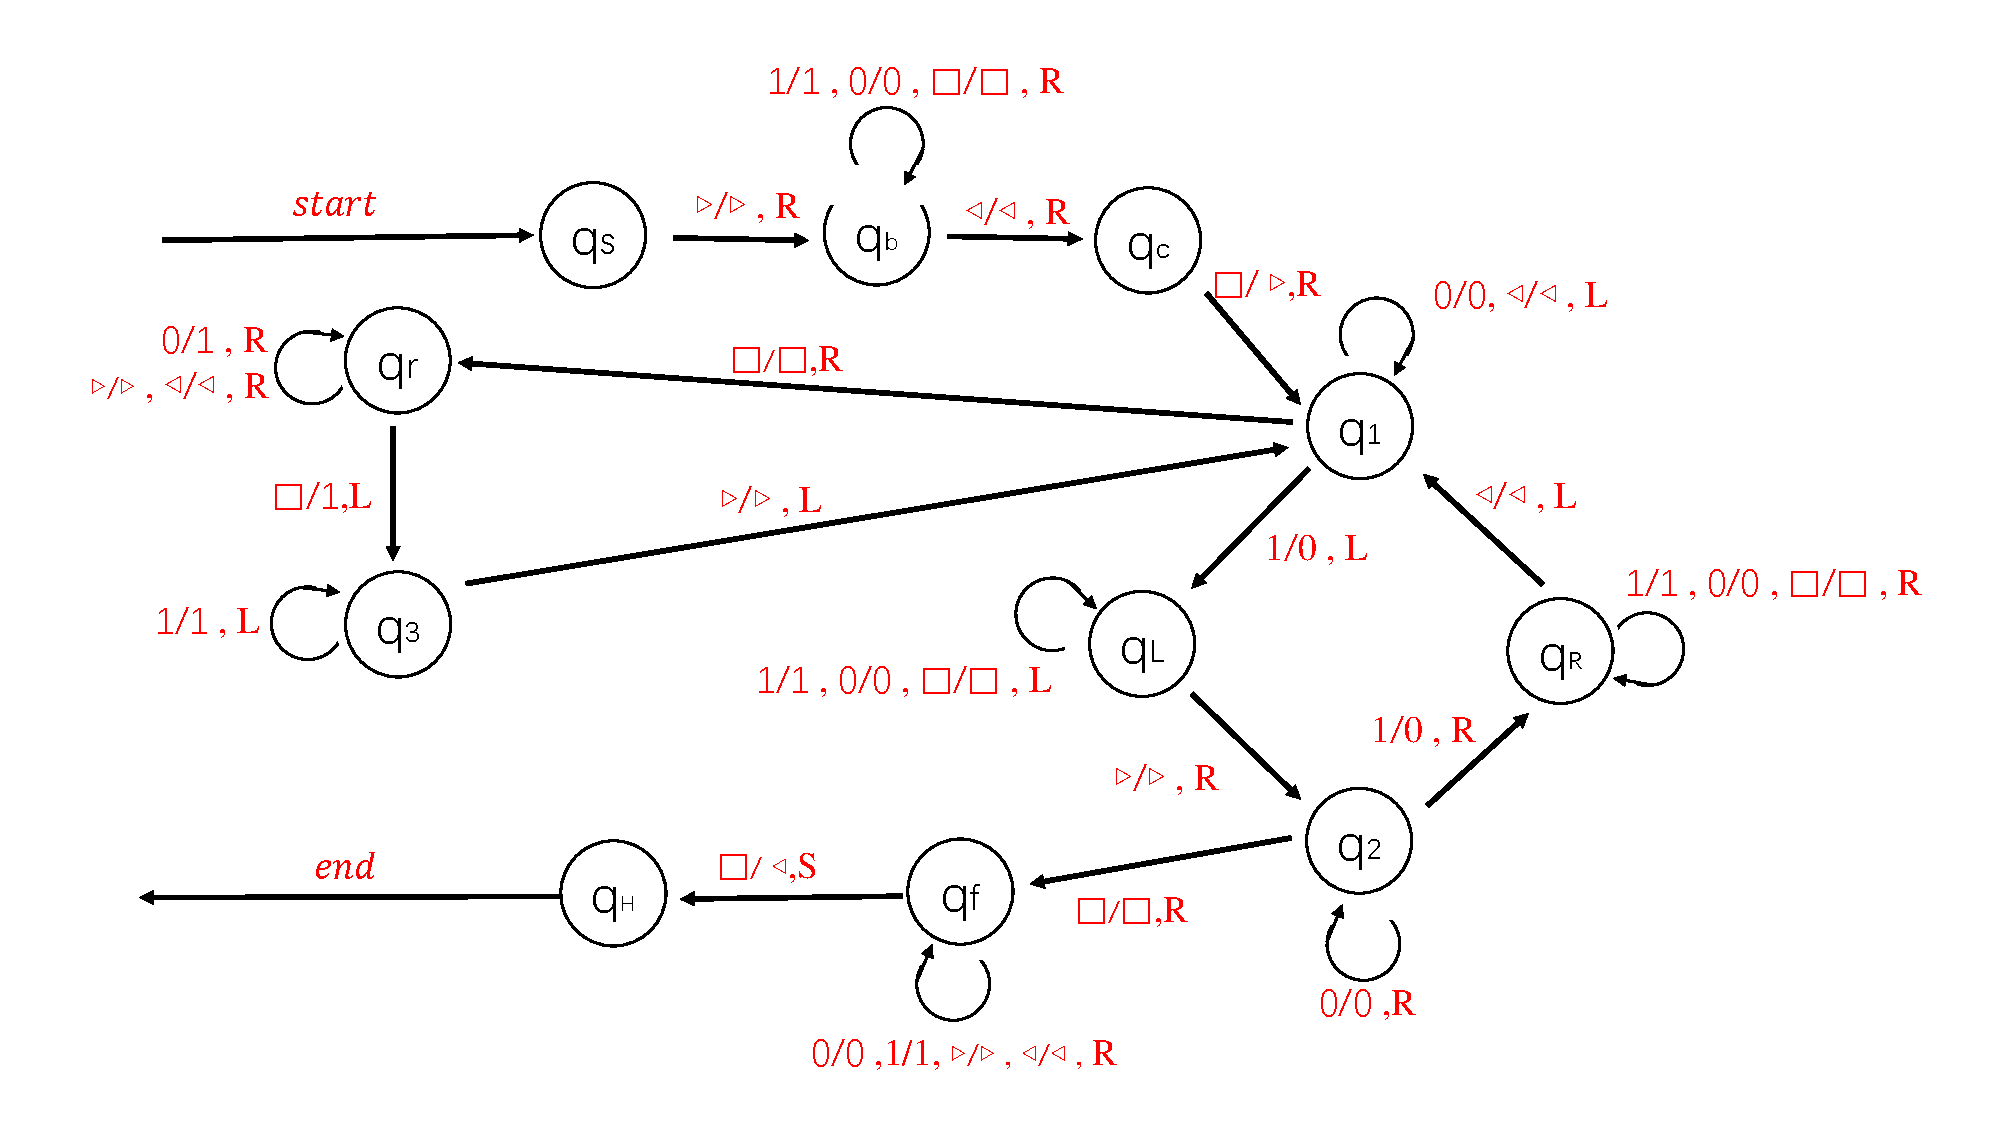
\includegraphics[width=1\textwidth]{turing machine.pdf}
        \caption{state transition diagram}\label{std}
        \end{figure}
        \item
        \begin{equation}
            \begin{aligned}
            (q_s,\underline{\triangleright}  1  1  1  1  1  1  1  \Box 1  1  1   \triangleleft)
	\vdash (q_b,\triangleright  \underline{1}  1  1  1  1  1  1  \Box 1  1  1   \triangleleft)
	\vdash(q_b,\triangleright  1  1  1  1  1  1  1 \Box 1  1  1   \underline{\triangleleft} )\\
	\vdash(q_c,\triangleright  1  1  1  1  1  1  1  \Box 1  1  1   \triangleleft \underline{~})
	\vdash(q_1,\triangleright  1  1  1  1  1  1  1 \Box 1  1  1    \underline{\triangleleft} \triangleright )\vdash(q_1,\triangleright  1  1  1  1  1  1  1 \Box 1  1  \underline{1}    \triangleleft \triangleright)\\
	First~round~~~~~~~~~~~~~~~~~~~~~~~~~~~~~~~~~~~~~~~~~~~~~~~~~~~~~~~~~~~~~\\
	\vdash(q_L,\triangleright  1  1  1  1  1  1  1 \Box 1  \underline{1}  0    \triangleleft \triangleright )\vdash(q_L,\underline{\triangleright}  1  1  1  1  1  1  1 \Box 1  1  0    \triangleleft \triangleright )\vdash(q_2,\triangleright  \underline{1}  1  1  1  1  1  1 \Box 1  1  0    \triangleleft \triangleright )\\
	\vdash(q_R,\triangleright  0  \underline{1}  1  1  1  1  1 \Box 1  1  0    \triangleleft \triangleright )\vdash(q_R,\triangleright  0  1  1  1  1  1  1 \Box 1  1  0    \underline{\triangleleft} \triangleright )\vdash(q_1,\triangleright  0  1  1  1  1  1  1 \Box 1  1  \underline{0}    \triangleleft \triangleright )\\
	\vdash(q_1,\triangleright  0  1  1  1  1  1  1 \Box 1  \underline{1}  0    \triangleleft \triangleright )\vdash(q_L,\triangleright  0  1  1  1  1  1  1 \Box \underline{1}  0  0    \triangleleft \triangleright )\vdash(q_L,\underline{\triangleright}  0  1  1  1  1  1  1 \Box 1  0  0    \triangleleft \triangleright )\\
	\vdash(q_2,\triangleright  \underline{0}  1  1  1  1  1  1 \Box 1  0  0    \triangleleft \triangleright )\vdash(q_R,\triangleright  0 \underline{0}    1  1  1  1  1 \Box 1  0  0    \triangleleft \triangleright )\vdash(q_R,\triangleright  0 0    1  1  1  1  1 \Box 1  0  0    \underline{\triangleleft} \triangleright )\\
	\vdash(q_1,\triangleright  0 0    1  1  1  1  1 \Box 1  0  \underline{0}    \triangleleft \triangleright )\vdash(q_1,\triangleright  0 0    1  1  1  1  1 \Box \underline{1}  0  0    \triangleleft \triangleright )\vdash(q_L,\triangleright  0 0    1  1  1  1  1 \underline{\Box} 0  0  0    \triangleleft \triangleright )\\
	\vdash(q_L,\underline{\triangleright}  0 0    1  1  1  1  1 \Box 0  0  0    \triangleleft \triangleright )	\vdash(q_2,\underline{\triangleright}  0 0    1  1  1  1  1 \Box 0  0  0    \triangleleft \triangleright )	\vdash(q_2,\triangleright  0 0    \underline{1}  1  1  1  1 \Box 0  0  0    \triangleleft \triangleright )\\
		\vdash(q_R,\triangleright  0 0    0  \underline{1}  1  1  1 \Box 0  0  0    \triangleleft \triangleright )		\vdash(q_R,\triangleright  0 0    0  1  1  1  1 \Box 0  0  0    \underline{\triangleleft} \triangleright )		\vdash(q_1,\triangleright  0 0    0  1  1  1  1 \Box 0  0  \underline{0}    \triangleleft \triangleright )\\
	\vdash(q_1,\triangleright  0 0    0  1  1  1  1 \underline{\Box} 0  0  0    \triangleleft \triangleright )\vdash(q_r,\triangleright  0 0    0  1  1  1  1 \Box \underline{0}  0  0    \triangleleft \triangleright )\vdash(q_r,\triangleright  0 0    0  1  1  1  1 \Box 1 1 1    \underline{\triangleleft} \triangleright )\\
	\vdash(q_r,\triangleright  0 0 0  1  1  1  1 \Box 1 1 1    \triangleleft \triangleright \underline{~})\vdash(q_3,\triangleright  0 0 0  1  1  1  1 \Box 1 1 1    \triangleleft \underline{\triangleright} 1)\vdash(q_1,\triangleright  0 0 0  1  1  1  1 \Box 1 1 1    \underline{\triangleleft} \triangleright 1)\\
	Second~round~~~~~~~~~~~~~~~~~~~~~~~~~~~~~~~~~~~~~~~~~~~~~~~~~~~~~~~~~~~~~\\
	\vdash(q_L,\triangleright  0 0 0  1  1  1  1 \Box 1  \underline{1}  0    \triangleleft \triangleright 1)\vdash(q_L,\underline{\triangleright}  0 0 0  1  1  1  1 \Box 1  1  0    \triangleleft \triangleright 1)\vdash(q_2,\triangleright  \underline{0}  0 01  1  1  1  1 \Box 1  1  0    \triangleleft \triangleright 1)\\
	\dots\dots~~~~~~~similar~to~the~First~round~~~~~~~~~~~~~~~~~~~~~~~~~~~~~~~~~~~~~~~~~~~~\\
	\vdash(q_1,\triangleright  0 0 0  0  0  0  1 \Box 0  0 \underline{0}      \triangleleft \triangleright 1)\vdash(q_1,\triangleright  0 0 0  0  0  0  1 \underline{\Box} 0  0 0      \triangleleft \triangleright 1)\vdash(q_r,\triangleright  0 0 0  0  0  0  1 \Box \underline{0}  0 0  \triangleleft \triangleright 1)\\
	\vdash(q_r,\triangleright  0 0 0  0  0  0  1 \Box 1 1 1\underline{\triangleleft}\triangleright 1)\vdash(q_r,\triangleright  0 0 0  0  0  0  1 \Box 1 1 1\triangleleft\triangleright 1\underline{~})\vdash(q_3,\triangleright  0 0 0  0  0  0  1 \Box 1 1 1\triangleleft\triangleright \underline{1} 1)\\
	\vdash(q_3,\triangleright  0 0 0  0  0  0  1 \Box 1 1 1\triangleleft\underline{\triangleright } 1 1)
	\vdash(q_1,\triangleright  0 0 0  0  0  0  1 \Box 1 1 1\underline{\triangleleft}\triangleright 1 1)
	\vdash(q_1,\triangleright  0 0 0  0  0  0  1 \Box 1 1 \underline{1}\triangleleft\triangleright 1 1)\\
	Third~round(unable~to~finish)~~~~~~~~~~~~~~~~~~~~~~~~~~~~~~~~~~~~~~~\\
	\vdash(q_L,\triangleright  0 0 0  0  0  0  1 \Box 1 \underline{1} 0\triangleleft\triangleright 1 1)\vdash(q_L,\underline{\triangleright}  0 0 0  0  0  0  1 \Box 1 1 0\triangleleft\triangleright 1 1)\vdash(q_2,\triangleright  \underline{0} 0 0  0  0  0  1 \Box 1 1 0\triangleleft\triangleright 1 1)\\
	\vdash(q_2,\triangleright  0 0 0  0  0  0  \underline{1} \Box 1 1 0\triangleleft\triangleright 1 1)
	\vdash(q_R,\triangleright  0 0 0  0  0  0  0 \underline{\Box} 1 1 0\triangleleft\triangleright 1 1)
	\vdash(q_R,\triangleright  0 0 0  0  0  0  0 \Box 1 1 0\underline{\triangleleft}\triangleright 1 1)\\
	\vdash(q_1,\triangleright  0 0 0  0  0  0  0 \Box 1 1 \underline{0}\triangleleft\triangleright 1 1)
	\vdash(q_1,\triangleright  0 0 0  0  0  0  0 \Box 1 \underline{1} 0\triangleleft\triangleright 1 1)
	\vdash(q_L,\triangleright  0 0 0  0  0  0  0 \Box \underline{1} 0 0\triangleleft\triangleright 1 1)
	\\
	\vdash(q_L,\underline{\triangleright}  0 0 0  0  0  0  0 \Box 1 0 0\triangleleft\triangleright 1 1)
	\vdash(q_2,\triangleright  \underline{0} 0 0  0  0  0  0 \Box 1 0 0\triangleleft\triangleright 1 1)
	\vdash(q_2,\triangleright  0 0 0  0  0  0  0 \underline{\Box} 1 0 0\triangleleft\triangleright 1 1)\\
	Ready~to~stop~~~~~~~~~~~~~~~~~~~~~~~~~~~~~~~~~~~~~~~~~~~~~~~~~~~~~~~~~~~~~\\
	\vdash(q_f,\triangleright  0 0 0  0  0  0  0 \Box \underline{1} 0 0\triangleleft\triangleright 1 1)
	\vdash(q_f,\triangleright  0 0 0  0  0  0  0 \Box 1 0 0\triangleleft\triangleright 1 1\underline{~})
	\vdash(q_H,\triangleright  0 0 0  0  0  0  0 \Box 1 0 0\triangleleft\triangleright 1 1 \underline{\triangleleft})
            \end{aligned}
        \end{equation}
    \end{enumerate}
\end{solution}
    \item 
    Given the alphabet $\{1, 0, \Box, \triangleright, \triangleleft\}$, design a time efficient 3-tape TM $M$ to compute $f:\{0,1\}^*\rightarrow\{0,1\}$ which verifies whether the number of 0 and the number of 1 are the same in an input consisting of only 0's and 1's. $M$ should output 1 if the numbers are the same, and 0 otherwise. For eample, for the input tape $\triangleright 001101\triangleleft$, $M$ should output 1
    
    \begin{enumerate}
	    \item
	    Please describe your design and then write the specifications of $M$ in the form like $\langle q_S, \triangleright, \triangleright, \triangleright \rangle \rightarrow \langle q_1, \triangleright,\triangleright,  R, R, S \rangle$. Explain the transition functions in detail.
	    
	    \item 
	    Show the time complexity for one-tape TM $M'$ to compute the same function $f$ with $n$ symbols in the input and give a brief description of such $M'$ .
	
	\end{enumerate}
	\begin{solution}
    \begin{enumerate}
        \item 
        Firstly, copy all the 0 from tape 1 to tape 2
        \begin{equation}
            \begin{aligned}
            <q_s,\triangleright,\triangleright,\triangleright> ~&\rightarrow~ <q_c,\triangleright,\triangleright,R,R,R>\\
            <q_c,0,\Box,\Box> ~&\rightarrow~ <q_c,0,\Box,R,R,S>\\
            <q_c,1,\Box,\Box> ~&\rightarrow~ <q_c,\Box,\Box,R,S,S>\\
            <q_c,\triangleleft,\Box,\Box> ~&\rightarrow~ <q_L,\triangleleft,\Box,L,L,S>\\
            \end{aligned}
        \end{equation}
        Secondly, move to the beginning of the tape
        \begin{equation}
            \begin{aligned}
            <q_L,1,0,\Box> ~&\rightarrow~ <q_L,1,0,L,L,S>\\
            <q_L,0,0,\Box> ~&\rightarrow~ <q_L,0,0,L,L,S>\\
            <q_L,1,\triangleright,\Box> ~&\rightarrow~ <q_L,1,\triangleright,L,S,S>\\
            <q_L,0,\triangleright,\Box> ~&\rightarrow~ <q_L,0,\triangleright,L,S,S>\\
            <q_L,\triangleleft,\triangleright,\Box> ~&\rightarrow~ <q_1,\triangleleft,\triangleright,R,R,S>\\
            \end{aligned}
        \end{equation}
        Thirdly, begin to compare,if read 1 in tape 1,move tape 2 an unit right,else do not move in tape 2.If read $1$ in tape 1 but $\triangleleft$ in tape 2(means ending in tape 2), output 0.
        If read $\triangleleft$ in tape 1 and tape 2 in the same time, output 1.
        \begin{equation}
            \begin{aligned}
            <q_1,0,0,\Box> ~&\rightarrow~ <q_1,0,0,R,S,S>\\
            <q_1,1,0,\Box> ~&\rightarrow~ <q_1,1,0,R,R,S>\\
            <q_1,0,\triangleleft,\Box> ~&\rightarrow~ <q_1,0,\triangleleft,R,S,S>\\
            <q_1,1,\triangleleft,\Box> ~&\rightarrow~ <q_f,1,\triangleleft,S,S,R>\\
            <q_1,\triangleleft,\triangleleft,\Box> ~&\rightarrow~ <q_f,\triangleleft,1,S,S,R>\\
            <q_1,\triangleleft,0,\Box> ~&\rightarrow~ <q_f,\triangleleft,0,S,S,R>\\
            \end{aligned}
        \end{equation}
        At last, end the Turing machine.($\forall$ means not caring what).Then we will get the output in tape 3.("$\triangleright 1\triangleleft$" or "$\triangleright 0\triangleleft$").
        \begin{equation}
            <q_f,\forall,\forall,\Box> ~\rightarrow~<q_H,\triangleleft,\triangleleft,S,S,S>
        \end{equation}
        \item
        \begin{enumerate}
            \item ~\par
            Except for the finishing state, we always moves in tape 1, so we only need to count the movement in tape 1.\\
        First we move from the beginning to the end and return to the beginning, which cost $2*n$ times.\\
        Then when comparing, we at most move the tape 1 from beginning to the end, which cost $n$ times.\\
        As a result, the time complexity is $O(n)$.
        \item 
        When there is only one tape, we have use the same idea but need more time.\\
        Firstly, we copy all the 0 to the end of the tape. We only need to marked the 0 that have been moved by changing it to $\Box$.Then we have 2 parts,one is the input, and the other is all the 0s, which are blocked by $\triangleright$.Every moving costs $2*n=O(n)$ time complexity.\\
        Secondly, during the comparing time, when reading an 1 in the first part, change a 0 into 1 in the 1 in the second part.If there is no 0 ready for changing or there are 0s left in the end , change to fail state to end, else change to success state to end.Every compare costs $2*n=O(n)$ time complexity\\
        Lastly, according to the state, output 1 or 0.As every operation cost $O(n)$ time complexity and we total need $O(n)$ operations (according to the method above), so the total time complexity is $O(n^2)$.
        \end{enumerate}
        \end{enumerate}
    \end{solution}
	\item Define the corresponding decision or search problem of the following problems and give the "certificate" and "certifier" for each decision problem provided in the subquestions or defined by yourself.
	
	\begin{enumerate}
	    \item
	    \textit{3-Dimensional Matching.}  Given disjoint sets $X,Y,Z$ all with the size of $n$, and a set $M \subseteq X\times Y\times Z$.  Is there a subset $M'$ of $M$ of size $n$ where no two elements of $M'$ agree in any coordinate?
	    
	    \item 
	    \textit{Travelling Salesman Problem.} Given a list of cities and the distances between each pair of cities, find the shortest possible route that visits each city exactly once and returns to the origin city.
	    
	    \item
	    \textit{Job Sequencing.} Given a set of unit-time jobs, each of which has an integer deadline and a nonnegative penalty for missing the deadline. Does there exist a job sequence that has a total penalty $w\leqslant k$?
	    
	\end{enumerate}
	\begin{solution}
	    \begin{enumerate}
	        \item This is a decision problem.\\
	        Certificate: A subset $M'$
	        ~\par
	  \begin{algorithm}[H]
		\KwIn{A set $M'$}
		\KwOut{$True$ or $False$}
		\BlankLine
		\caption{3-Dimensional Matching certifier}\label{3D}
		\For{$a\in M'$}{
		\For{$b\in M'$}{
		    \If{$a\neq b$}{
		    \If{$a_x==b_x ||a_y==b_y|| a_z==b_z$}{
		    \Return False}
		    }
		}
		}
		\Return True
	\end{algorithm}
	We can define corresponding search problem that Given $X,Y,Z,M$,\\1)find the subset $M'$ of $M$ that of the largest size \\or 2)find a subset $M'$ of $M$ of size $n$ if it exists
	\item This is a search problem. When can define the decision problem that If there is a route S that its weight is no larger than $k$.\\
	Certificate: A route $S$\\
	\begin{algorithm}[H]
		\KwIn{A route $S$,range $k$}
		\KwOut{$True$ or $False$}
		\BlankLine
		\caption{Travelling Salesman Problem.}\label{TSP}
		\If{route S visits each city exactly once and returns to the origin city}{
		$a\leftarrow 0$\\
		\For{$edge\in S$}{
		$a\leftarrow a+weight(edge)$
		}
		\If{$a<=k$}{
		\Return True
		}
		}
		\Return False
	\end{algorithm}
	\item 
	This is a decision problem.\\
	Certificate: A Job sequence $S$\\
	\begin{algorithm}[H]
		\KwIn{A Job sequence $S$,range $k$}
		\KwOut{$True$ or $False$}
		\BlankLine
		\caption{Job Sequencing.}\label{JS}
		$\omega\leftarrow 0$\\
		\For{$job\in S$}{
		$\omega\leftarrow \omega+penalty(job)$
		}
		\If{$\omega<=k$}{
		\Return True
		}
		\Else{\Return False}
	\end{algorithm}
	We can define the search problem that find the job sequence $S'$ with the least penalty.
	    \end{enumerate}
	\end{solution}
\end{enumerate}

\textbf{Remark:} Please include your .pdf, .tex files for uploading with standard file names.
\newpage


%========================================================================
\end{document} 